% Chapter 2
\chapter{مفاهیم پایه}
\thispagestyle{empty}
\section{مقدمه}
در این قسمت به بررسی‌ و توضیح  مفاهیم پایه مورد نیاز در بحث مدل‌سازی موضوع
و آنالیز احساس\LTRfootnote{Sentiment Analysis}
می‌‌پردازیم. در ابتدا بر روی مفاهیم ریاضی‌ و مدل‌های احتمالاتی\LTRfootnote{Probabilistic Model}،
   انواع و تفاوت‌های آنها تمرکز می‌‌کنیم، سپس در مورد توابع ریاضی مورد نیاز در بخش‌های بعدی توضیح داده می‌شود و در 
ادامه با مفاهیم موجود در حوزه‌ی مدل‌سازی موضوعی و کاوش عقاید\LTRfootnote{Opinion Mining}
 آشنا می‌‌شویم و در مورد هر کدام توضیحات مورد نیاز را ارائه می‌‌دهیم. 

\section{متغیر مشاهده شده و متغیر پنهان }
در علم آمار\LTRfootnote{Statistic}
و احتمال متغیر مشاهده شده\LTRfootnote{Observed Variable}
به متغیری گفته می‌‌شود که مقدار آن واقعا مشاهده شده باشد و یا واقعا اتفاق افتاده باشد. در مقابل آن متغیر مخفی‌ یا پنهان\LTRfootnote{Latent Variable}
وجود دارد که به متغیری گفت می‌‌شود که از دیگر متغیر‌های مشاهده شده استنتاج\LTRfootnote{Inference}
 می‌‌شود.

\section{مدل‌ احتمالاتی}
به زبان ساده، یک مدل احتمالی‌ که به آن مدل آماری\LTRfootnote{Statistical Model}
نیز می‌‌گویند، دسته‌ای‌ از مدل‌های ریاضی‌ است که با مجموعه‌ای از فرضیات  همراه است که بر روی تولید داده‌های نمونه\LTRfootnote{Sample Data}
و یا داده‌های مشابه از یک جمعیت بزرگتر یا از یک سیستم تمرکز می‌‌کنند. فرضیاتی که در اینجا در مورد آن صحبت می‌‌کنیم و همراه با یک مدل احتمالی‌ هستند در واقع توزیع‌های احتمالاتی\LTRfootnote{Probabilistic Distribution}
هستند که احتمال رخداد یا تولید نمونه‌های مختلف از جمعیت بزرگتر را برای ما مشخص می‌‌کنند. به بیان دیگر مدل احتمالی‌ به مدلی‌ گفته می‌‌شود که داده‌هایی که می‌‌توانند از یک سیستم مشاهده شوند را برای ما توصیف می‌‌کند.

به بیان ریاضی‌، یک مدل احتمالی‌ به صورت یک جفت به شکل
$(S,P)$
در نظر گرفته می‌‌شود که در آن
$S$
مجموعه‌ی تمام مشاهدات ممکن یا به عبارت دیگر همان فضای نمونه\LTRfootnote{Sample Space}
 و
$P$
مجموعه‌ی توزیع‌های احتمالاتی بر روی
$S$
می‌ باشد. در این تعریف فرض بر این است که یک توزیع احتمالاتی درست منجر به تولید داده‌های قابل مشاهده گردیده است. ما
$P$
را به عنوان مجموعه‌ای از توزیع‌های احتمالاتی انتخاب می‌‌کنیم که به اندازه‌ی کافی‌ این توزیع احتمالی‌ درست را با دقت مناسب تقریب بزنیم.

مدل‌های احتمالی‌ را از نظر توزیع احتمالی‌ که سعی‌ در تقریب زدن آن به شکلی‌ مناسب و با دقت کافی‌ دارند را می‌‌توان در دو دسته کلی‌ مدل‌های مولد\LTRfootnote{Generative Models}
و مدل‌های افتراقی\LTRfootnote{Discriminative Models}
 دسته‌بندی کرد، که در ادامه به توضیح هرکدام از این دو دسته می‌‌پردازیم و آن‌ها را با یکدیگر مقایسه می‌‌کنیم.

	\subsection{مدل‌ احتمالاتی افتراقی}
	مدل‌های افتراقی که همچنین از آن‌ها به عنوان مدل‌های شرطی\LTRfootnote{Conditional Models}
	نیز یاد می‌‌شود یک کلاس از مدل‌های احتمالی‌ است که بیشتر در مباحث مربوط به یادگیری ماشین\LTRfootnote{Machine Learning}
	برای مدل کردن وابستگی یک متغیر مشاهده نشده مانند
	$y$
	به یک متغیر مشاهده شده مانند
	$x$
	مورد استفاده قرار می‌‌گیرند. در یک مدل افتراقی
	$p(y|x)$
	که یک توزیع احتمالی‌ شرطی است مدل می‌‌شود و می‌‌توان از آن برای پیش‌بینی‌
	$y$
	با توجه به
	$x$
	استفاده کرد.
	
	برای کاربردهایی مانند طبقه‌بندی
	و رگرسیون\LTRfootnote{Regression}
	که در آن‌ها از احتمالات شرطی استفاده می‌‌کنیم مدل‌های افتراقی نسبت به مدل‌های دیگر نتایج بهتری را از خود نشان می‌‌دهند. علاوه بر این مدل‌های افتراقی به صورت ذاتی در دسته مدل‌های نظارت‌شده\LTRfootnote{Supervised}
	قرار می‌‌گیرند و به آسانی‌ قابل بسط دادن به حالت بدون نظارت
	ناست. مدل هایی مانند: ماشین‌های بردار پشتیبان\LTRfootnote{Support Vector Machine}،
	 شبکه‌های عصبی\LTRfootnote{ٔNeural Networks}، 
	 رگرسیون خطی‌\LTRfootnote{Linear Regression}
	  و غیره که در یادگیری ماشین از آن‌ها استفاده می‌‌کنیم در دسته‌ی مدل‌های افتراقی قرار می‌‌گیرند.
	
	\subsection{مدل‌ احتمالاتی مولد}
	\label{chap2sec3sub2}
	مدل‌های احتمالی‌ مولد در مقابل مدل‌های احتمالی‌ افتراقی قرار دارند و در مسائل یادگیری پیچیده از انعطاف پذیری بیشتری نسبت به مدل افتراقی برخوردارند. به طور کلی‌ در مباحث آماری و احتمالاتی، یک مدل مولد به مدلی‌ گفت می‌‌شود که با در نظر گرفتن تعدادی متغیر پنهان داده شده، داده‌های قابل مشاهده را تولید می‌‌کند. اساس کار مدل‌های مولد توزیع احتمالی‌ مشترک\LTRfootnote{Joint Probability Distribution}
	است. این مدل‌ها نیز همانند دسته‌ی پیشین در مباحث مربوط به یادگیری ماشین به دو شکل کلی‌ مورد استفاده قرار می‌‌گیرند. ۱) برای مدل کردن داده‌ها به صورت مستقیم یا به عبارت دیگر مدل کردن داده‌های قابل مشاهده که از یک تابع چگالی احتمال\LTRfootnote{Probability Density Function}
	بدست می‌‌آیند. ۲) به عنوان یک مرحله‌ی میانی برای تشکیل یک تابع چگالی احتمال شرطی\LTRfootnote{Conditional Probability Density Function}
	که با استفاده از قانون بیز\LTRfootnote{Bayes Rule}
	 ساخته می‌‌شوند مورد استفاده قرار میگیرند.
	
	یک مدل مولد، یک مدل احتمالاتی کامل بر اساس تمام متغیر‌ها است. در حالی‌ که یک مدل افتراقی، تنها یک مدل مشروط برای متغیر هدف\LTRfootnote{Target Variable}
	بر اساس متغیر‌های قابل مشاهده را مهیا می‌‌کند، لذا از این نظر مدل‌های افتراقی و مولد کاملا در مقابل یکدیگر قرار دارند. در نتیجه مدل‌های مولد برای مواردی نظیر شبیه‌سازی یا تولید هر یک از متغیر‌ها در یک مدل می‌‌توانند مورد استفاده قرار بگیرند، در حالی‌ که مدل‌های افتراقی تنها اجازه‌ی نمونه‌برداری\LTRfootnote{Sampling}
	از متغیر هدف مشروط به مقادیر قابل مشاهده را می‌‌دهند. خصوصیات بیان شده برای مدل‌های مولد باعث می‌‌شود که این مدل به نتایج بهتری در مسائل بدون نظارت  دست یابند. مدل‌هایی مانند: مدل مخلوط گوسی\LTRfootnote{Gaussian Mixture Model}، مدل مخفی‌ مارکوف\LTRfootnote{Hidden Markov Model}، تخصیص دیریکله‌ی پنهان\LTRfootnote{Latent Dirichlet Allocation}
	که در فصل بعدی به صورت کامل توضیح داده می‌‌شود و ماشین بلتزمن محدود\LTRfootnote{Restricted Boltzman Machine}
	که در فصل مدل پیشنهادی از آن استفاده می‌کنیم در دسته‌ی مدل‌های مولد قرار می‌‌گیرند.
\section{مدل گرافی}
\label{chap2sec4}
مدل‌های گرافی\LTRfootnote{Graphical Model}
یا مدل‌های گرافی احتمالاتی، دسته‌ای از مدل‌های احتمالاتی هستند که در حالت کلی‌ برای نمایش وابستگی شرطی بین متغیر‌های تصادفی در آن‌ها، از یک نمودار گراف مانند استفاده می‌‌کنند. کاربرد اصلی‌ این مدل‌ها در بحث تئوری آمار و احتمال (بخصوص آمار و احتمال بیزی) و یادگیری ماشین است.

در شکل
\ref{chap2-fig4}
یک نمونه از مدل‌های گرافی‌ را مشاهده می‌‌کنید. در این شکل و به طور کلی‌ در این مدل‌ها، مستطیل‌ها نشان دهنده‌ی تکرار و تعداد هستند. پیکان‌های جهتدار وابستگی‌های شرطی را نشان می‌‌دهند و دایره‌ها نشان دهنده‌ی متغیر‌های تصادفی هستند. متغیر‌های تصادفی می‌‌توانند سفید‌ (پنهان و مشاهده نشده) و یا تیره (متغیر‌های قابل مشاهده) باشند.
\begin{figure}[!t]
	\centering
	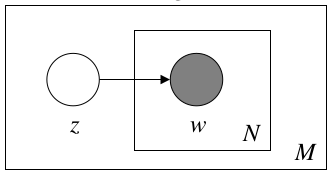
\includegraphics[scale=0.5]{chap2-img/graphicalmodel}
	\caption{نمومه‌ای از یک مدل گرافی \cite{blei2003latent}}
	\label{chap2-fig4}
\end{figure}

برای مثال در شکل
\ref{chap2-fig4}
که یک مدل گرافی ساده را نشان می‌‌دهد، مستطیل بیرونی
$M$
بار و مستطیل درونی به ازای هر بار تکرار مستطیل بیرونی
$N$
بار تکرار می‌‌شود. همچنین این مدل از دو متغیر تصادفی تشکیل شده که بین آن‌ها یک وابستگی شرطی نیز وجود دارد و یکی‌ از آن‌ها یک متغیر پنهان
($z$)
و دیگری یک متغیر قابل‌مشاهده
($w$)
می‌ باشد.
\section{مدل مخلوط}
در علم آمار یک مدل مخلوط\LTRfootnote{Mixture Model}
یک مدل احتمالاتی است که از آن برای نشان دادن وجود چند زیر جامعه\LTRfootnote{Subpopulation}
در یک جامعه‌ی بزرگتر بدون نیاز به داده‌ی قابل مشاهده برای شناسایی‌ و تشخیص آن زیر جامعه‌ها استفاده می‌‌‌شود. به بیان رسمی‌، یک مدل مخلوط متناظر با یک توزیع مخلوط\LTRfootnote{Mixture Distribution}
 است که توزیع‌های احتمالاتی مشاهده شده در یک جامعه‌ی کلی‌ یا جمعیت بزرگتر را نشان می‌‌دهد.
	
\section{تابع لجستیک}
تابع لجستیک\LTRfootnote{Logistic Function}
 یک منحنی متداول از خانواده‌ی منحنی‌های سیگمویدی\LTRfootnote{Sigmoid Curves}
  است. معاد‌له‌ی:
\begin{align}
	f(x) = \frac{L}{1+e^{-k(x-x_0)}}
	\label{eq1}
\end{align}
نشان دهنده یک تابع لجستیک است که در آن
$x_0$
نقطه میانی منحنی سیگمویدی روی محور
x
ها،
$L$
مقدار بیشینه منحنی در مثبت بی‌ نهایت و
$k$
برابر با شیب منحنی است.


 در شکل
\ref{fig3}
برای مقادیر x در بازه‌ی اعداد حقیقی‌ از منفی‌ بی‌ نهایت تا مثبت بی‌ نهایت نمودار این منحنی نشان داده شده است. تابع لجستیک در ادامه برای معرفی تابع
softmax
مورد استفاده قرار می‌‌گیرد.
\begin{figure}[!h]
	\centering
	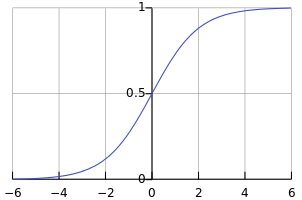
\includegraphics[scale=0.5]{chap2-img/logistic_function}
	\caption{تابع لجستیک در بازه‌ی اعداد حقیقی‌ از منفی‌ بی‌ نهیات تا مثبت بی‌ نهیات }
	\label{fig3}
\end{figure}

\section{تابع Softmax}
\label{chap2sec9}
در ریاضیات تابع
Softmax
که به آن تابع توانی‌ نرمال‌شده\LTRfootnote{Normalized Exponential Function}
 نیز می‌‌گویند، یک تابع لجستیک تعمیم یافته است که از آن برای نرم کردن یک بردار
K
بعدی مانند
\textbf{z}
متشکل از اعداد حقیقی‌ دلخواه به یک بردار
K
بعدی مانند
$\sigma(\textbf{z})$ 
تشکیل شده از اعداد حقیقی‌ بین بازه‌ی
$(0,1)$
به گونه‌ای که مجموع آنها برابر با ۱ باشد استفاده می‌‌کنند. رابطه‌ی:
\begin{align}
	\sigma(\textbf{z}) = \frac{e^{z_i}}{\sum_{k=1}^{K}e^{z_k}} \quad\quad for\quad i = 1, ..., K
	\label{eq2}
\end{align}
معادله‌ی تابع
Softmax
را نشان می‌‌دهد. با توجه به خاصیت ذکر شده برای بردار حاصل از تابع
Softmax
در تئوری احتمال از این خروجی برای تعریف یک توزیع احتمالی که دارای
K
خروجی ممکن است استفاده می‌کنند. در بخش‌های بعدی از این تابع برای تعریف توزیع‌های احتمالی‌ برای موضوعات مختلف استفاده می‌‌کنیم.


\section{تابع گاما}
\label{chap2sec8}
تابع گاما\LTRfootnote{Gamma Function}
 که آن را با
$\Gamma$
نشان می‌‌دهند از تابع فاکتوریل مشتق شده است و برای یک عدد صحیح مثبت مقدار آن از رابطه:
\begin{align}
	\centering
	\label{eq13}
	\Gamma(n) = (n-1)!
\end{align}
بدست می‌‌آید. تابع گاما در واقع برای تمام اعداد نامنفی حتی اعدد مختلظ نیز تعریف می‌‌شود. برای یک عدد مختلط با بخش حقیقی مثبت مقدار این تابع از رابطه
\begin{align}
	\centering
	\label{eq14}
	\Gamma(z) = \int_{0}^{\infty} x^{z-1}e^{-x}dx
\end{align}
بدست می‌‌آید.

\section{زنجیره‌ی مارکوف مونت کارلو}
\label{chap2sec6}
روش زنجیره‌ مارکوف مونت کارلو\LTRfootnote{Markov Chain Mont Carlo}
 که به اختصار آن را
MCMC
می‌ گویند، در کلاس روش‌های تولید نمونه از یک توزیع احتمالاتی قرار دارد. به زبان خیلی‌ ساده
MCMC
با ساختن یک زنجیر مارکوف برگشت‌پذیر\LTRfootnote{Reversible}
که در حالت تعادل توزیعی مشابه توزیع مورد نظر ما را دارد، از توزیع احتمالاتی نمونه تولید می‌‌کند. به بیان دیگر حالت زنجیر مارکوف، بعد از طی‌ کردن چند مرحله به عنوان یک نمونه از توزیع احتمالاتی مورد نظر در نظر گرفته می‌شود. کیفیت نمونه‌‌ی تولید شده توسط روش
MCMC
با تعداد مراحلی که زنجیر مارکوف اجرا می‌‌گردد رابطه‌ی مستقیم دارد و هرچه تعداد این مراحل بیشتر باشد نمونه‌ی بهتری بدست خواهد داد.

\section{الگوریتم یادگیری واگرایی مقابله}
\label{chap2sec7}
الگوریتم یادگیری واگرایی مقابله\LTRfootnote{Contrastive Divergence}
 اولین بار در سال ۲۰۰۲ توسط آقای هینتون
\cite{hinton2002training}
به عنوان یک الگوریتم یادگیری تقریبی بیشینه‌سازی مورد انتظار\LTRfootnote{Maximum Likelihood Approximation}
پیشنهاد گردید که در اینجا آن را به طور کامل توضیح می‌‌دهیم، و در ادامه خواهیم دید که پایه و اساس روش‌های یادگیری مدل‌های پیشین و پیشنهادی در این پایان‌‌نامه بر اساس همین الگوریتم هستند.

\subsection{الگوریتم واگرایی مقابله چیست و چرا به آن احتیاج داریم}
\label{chap2sec7sub1}

فرض کنید که قصد مدل‌سازی احتمال یک نقطه داده\LTRfootnote{Data Point}
 مانند
$x$
را با استفاده از یک تابع به شکل
$f(x;\theta)$
که در آن
$\theta$
یک بردار از پارامتر‌های مدل است را داریم. می‌‌دانیم که احتمال
$x$
که آن را به صورت
$p(x;\theta)$
نمایش می‌‌دهیم به ازای مجموع تمام حالت‌های
$x$
باید برابر با ۱ شود. بنابراین داریم:
\begin{align}
\centering
p(x;\theta) = \dfrac{1}{Z(\theta)}f(x;\theta)
\label{eg3}
\end{align}

که در آن
$Z(\theta)$
تابع قسمت‌بندی\LTRfootnote{Partition Function}
 است و به فرم
\begin{align}
\centering
Z(\theta) = \int f(x;\theta)dx
\label{eg4}
\end{align}
تعریف می‌شود. تابع قسمت‌بندی برای ما تضمین می‌‌کند که مقدار بدست آمده برای عبارت سمت چپ رابطه‌ی
\ref{eg3}
یک مقدار صحیح احتمالی‌ (بین ۰ و ۱) است
\cite{woodfordnotes}.

مجموعه پارامتر‌های مدل را که در اینجا با
$\theta$
نشان می‌‌دهیم، را با بیشینه کردن احتمال یک مجموعه‌‌ی آموزش\LTRfootnote{Training Set}
 از داده‌ها که آن را به صورت
$\textbf{X} = x_{1,...,K}$
تعریف می‌‌کنیم، یاد می‌‌گیریم. که در این حالت احتمال مجموعه آموزش از رابطه‌ی
\begin{align}
	\centering
	p(\textbf{X};\theta) = \prod_{k=1}^{K} \frac{1}{Z(\theta)} f(x_k;\theta)
	\label{eq5}
\end{align}
بدست می‌‌آید. یا با کمینه کردن مقدار منفی لگاریتم
$p(\textbf{X};\theta)$
که آن را با
$E(\textbf{X};\theta)$
نشان داده و انرژی مربوط به مدل تعریف می‌کنیم و از رابطه‌ی 
\begin{align}
	\centering
	E(\textbf{X};\theta) = \log Z(\theta) - \dfrac{1}{K} \sum_{i=1}^{K} \log f(x_i;\theta)
	\label{eq6}
\end{align}
محاسبه می‌شود، اقدام به یاد گیری پارامتر‌های مدل می‌‌کنیم.


در ادامه بر اساس نحوه‌ی تعریف تابع مدل احتمال، سه‌ حالت مختلف را بررسی‌ می‌‌کنیم و شرح می‌‌دهیم که الگوریتم یادگیری مقابله چیست، چرا و در چه حالتی به آن نیاز داریم.

اول حالتی را در نظر بگیرید که در آن تابع مدل احتمال\LTRfootnote{Probability Model Function}
 که آن را با
$p(x;\theta)$
نشان دادیم، تابع چگالی احتمال یک توزیع نرمال\LTRfootnote{Normal Distribution}
 به شکل
$N(x;\mu,\sigma)$
باشد. در این صورت مجموعه پارامتر‌های ما
$\theta = \{\mu,\sigma\}$
خواهد بود. بدیهی‌ است که انتگرال این تابع چگالی احتمال برابر با ۱ است. در نتیجه
$\log Z(\theta)=0$
می‌ شود. همچنین مشتق رابطه‌ی
\ref{eq6}
نسبت به
$\mu$
نشان می‌‌دهد که مقدار بهینه برای این متغیر
برابر با میانگین داده‌های آموزش است. همچنین مشتق رابطه‌ی
\ref{eq6}
این بار نسبت به
$\sigma$
نشان می‌‌دهد که مقدار بهینه برای این متغیر برابر با ریشه‌ی دوم واریانس داده‌های آموزش است.

در بعضی‌ مواقع مانند آنچه که در اینجا ذکر کردیم، روشی‌ وجود دارد که به صورت دقیق توانایی کمینه کردن تابع انرژی را دارد. برای درک بهتر، اگر تابع انرژی را در فضای پارامتر‌های مساله به صورت یک زمین مواج\LTRfootnote{Undulating Field}
در نظر بگیرید که هدف ما پیدا کردن پایین‌ترین نقطه در آن است، در این  صورت حالتی که در اینجا ذکر شد برابر است با زمانی‌ که در این زمین مواج همه چیز واضح و هوا آفتابی است و ما پایین‌ترین نقطه را مشاهده می‌‌کنیم و مستقیماً به سمت آن قدم می‌‌زنیم
\cite{woodfordnotes}.

برای حالت بعدی زمانی‌ را تصور کنید که در آن تابع مدل احتمال، برابر با مجموع
N
توزیع نرمال به شکل
\begin{align}
	\centering
	f(x;\theta)=\sum_{i=1}^N N(x;\mu_i,\sigma_i)
	\label{eg7}
\end{align}
باشد.
در این حالت مجموعه پارامترهای مدل به شکل
$\theta = \{\mu_{1,...,N},\sigma_{1,...,N} \}$ 
خواهد بود. این حالت مشابه زمانی‌ است که ما یک مدل مخلوط یا مجموعه‌ای از خبره‌ها 
\LTRfootnote{Mixture of Expert}
داشته باشیم که در آن وزن تمام افراد خبره برابر است. با توجه به این‌که انتگرال توزیع نرمال برابر با ۱ است، از رابطه
\ref{eg4}
داریم
$\log Z(\theta) = \log N$.
 در این حالت مشتق گرفتن از رابطه
\ref{eq6}
نسبت به هر یک از پارامتر‌های مدل، مدل جدیدی که وابسته به دیگر پارامتر‌های مدل است را تولید می‌‌کند. بنابراین مقدار بهینه برای پارامتر‌های مدل را به صورت مستقیم نمی‌‌توانیم محاسبه کنیم. راه جایگزین در این حالت استفاده از معادلات مشتقات جزئی‌ \LTRfootnote{Partial Differential}
و روش نزول گرادیانی\LTRfootnote{Gradient Descent}
 با جستجوی خطی‌\LTRfootnote{Line Search}
  است، که با استفاده از آن‌ها می‌‌توانیم نقطه کمینه محلی برای انرژی در فضای پارامتر‌های مدل را پیدا کنیم.

اگر به مثال خود برای حالت قبل باز گردیم، شرایط بیان شده در اینجا، یعنی‌ استفاده از نزول گرادیانی به همراه جستجوی خطی‌ مشابه زمانی‌ است که ما در هنگام شب به همراه یک مشعل در آن زمین مواج حضور داشته باشیم. همچنین ما توانایی احساس شیب نقطه‌ای که در آن ایستاده‌ایم را خواهیم داشت، یا می‌‌توانیم شیب این نقطه را نسبت به تمام جهت‌های اطرافمان تا فاصله‌ی اندکی‌ با استفاده از نور مشعل تعیین کنیم. بنابراین با تاباندن نور مشعل به جهتی‌ که برای حرکت انتخاب کرده‌ایم می‌‌توانیم پایین‌ترین نقطه در آن جهت را مشاهده کنیم به آن‌جا رفته و سپس جهت جدیدی را برای حرکت انتخاب کنیم
 \cite{woodfordnotes}.

 
 
 برای حالت سوم که حالت پایانی نیز است فرض کنید که ما تابع مدل احتمال را به صورت ضرب
 $N$
 توزیع نرمال به شکل
 \begin{align}
 	\centering
 	f(x;\theta)=\prod_{i=1}^N N(x;\mu_i,\sigma_i)
 	\label{eq8}
 \end{align}
 در نظر می‌‌گیریم.
این شرایط هم ارز با یک مدل ضرب خبره‌ها است. در این حالت تابع قسمت‌بندی دیگر مقدار ثابتی نخواهد داشت و بسته به مقادیر پارامتر‌های توزیع‌های نرمال مقدار آن متفاوت خواهد بود. برای مثال زمانی‌ که مدل فقط شامل دو توزیع نرمال است و برای هر دوی آن‌ها
 $\sigma = 1$
 را در نظر بگیرید. اگر
 $\mu_1 = -\infty$
 و
 $\mu_2 = \infty$
 آنگاه
 $Z(\theta) = 0$
 می‌ شود. در حالی‌ که اگر
 $\mu_1 = \mu_2 = 0$
 آنگاه
 $Z(\theta) = \frac{1}{2}\sqrt{\pi}$
 می‌شود. بنابراین بسته به مقادیری که برای پارامتر‌های مدل انتخاب می‌‌شوند مقدار
 $Z(\theta)$
 متغیر خواهد بود.
 
 اگرچه در این حالت محاسبه‌‌ی دقیق تابع قسمت‌بندی امکان پذیر است، اما شرایطی را در نظر بگیرید که در آن تابع مدل احتمال به گونه‌ای باشد که محاسبه‌ی‌ انتگرال در رابطه
\ref{eg4}
 از نظر جبری غیرعملی\LTRfootnote{Intractable}
 ‌ باشد. در این حالت برای ارزیابی رابطه
\ref{eq6}
 ما نیاز خواهیم داشت از انتگرال‌گیری عددی\LTRfootnote{Numerical Integration}
 استفاده کنیم. همچنین باید از مشتقات متناهی برای محاسبه گرادیان در یک نقطه‌ی داده شده در فضای پارامتر‌های مساله و همچنین روش‌های نزول گرادیانی برای پیدا کردن کمینه محلی استفاده کنیم. برای فضاهای داده‌ای و پارامتری با ابعاد بالا زمان این انتگرال‌گیری فلج کننده\LTRfootnote{Crippling}
 خواهد بود. شرایط بیان شده تا اینجا منجر به وضعیتی می‌‌گردد که در آن ما تلاش می‌‌کنیم یک تابع انرژی را کمینه کنیم در حالی‌ که توانایی ارزیابی کردن آن را نداریم.
 
 اینجا زمانی‌ است که الگوریتم واگرایی مقابله به ما کمک می‌‌کند. اگر چه که ما نمی‌‌توانیم خود تابع انرژی را ارزیابی کنیم اما الگوریتم
 CD
 برای ما راهی‌ را مهیا می‌‌کند که می‌توانیم به کمک آن گرادیان تابع انرژی را تخمین بزنیم. اگر به مثال خود برای حالت‌های قبل بازگردیم، در شرایط بیان شده برای حالت نهایی ما خودمان را در همان زمین مواج بدون هیچ‌گونه امکانات و توانایی خاصی خواهیم یافت (ما نمی‌‌توانیم انرژی را محاسبه کنیم)، در نتیجه ما امکان تشخیص ارتفاع و شیب در هیچ یک از نقطه‌های اطرافمان را نسبت به نقطه‌ای که در آن ایستاده‌ام را نداریم. الگوریتم
 CD
 در این حالت به ما یک حس تعادل می‌‌دهد و به ما این اجازه را می‌‌دهد که شیب نقطه‌ای از زمین که در زیر پایمان قرار دارد را تشخیص دهیم. حال با برداشتن قدم‌های بسیار کوچک در جهتی‌ که بیشترین کاهش شیب را داریم ما توانایی پیدا کردن راه خودمان به سمت کمینه‌ی محلی را خواهیم داشت
 \cite{woodfordnotes}.
 
\subsection{الگوریتم واگرایی مقابله چگونه کار می‌کند}
همان طور که در بخش
\ref{chap2sec7sub1}
توضیح داده شد، الگوریتم
CD
با توجه مجموعه پارامترهای مدل و داده‌های آموزش، گرادیان تابع انرژی را برای ما تخمین می‌‌زند.  در رابطه‌ی
\begin{align}
	\centering
	\label{eq9}
	\dfrac{\partial E(\textbf{X};\theta)}{\partial \theta} &= \dfrac{\log Z(\theta)}{\partial \theta} - \dfrac{1}{K}\sum_{i=1}^K\dfrac{\partial \log f(x_i;\theta)}{\partial \theta}\\\nonumber
	&= \dfrac{\log Z(\theta)}{\partial \theta} - \left\langle \dfrac{\partial \log f(x_i;\theta)}{\partial \theta}\right\rangle_\textbf{X}
\end{align}
 با استفاده از مشتقات جزئی فرمول محاسبه‌ی گرادیان را از را رابطه
\ref{eq6}
 بدست می‌‌آوریم. در رابطه‌ی
\ref{eq9}
 نماد
$\langle \star \rangle_\textbf{X}$
 نشان دهنده مقدار مورد انتظار برای
$\star$
 با توجه به توزیع داده‌ی
\textbf{X}
 می‌ باشد.

اولین ترم در سمت راست رابطه‌‌ی
\ref{eq9}
از تابع قسمت‌بندی مشتق می‌گردد و همانطور که در رابطه‌ی
\ref{eg4}
مشاهده می‌‌گردد شامل یک انتگرال‌گیری بر روی
$x$
است. با جایگذاری این رابطه به رابطه‌ی
\begin{align}
	\centering
	\label{eq10}
	\dfrac{\partial\log Z(\theta)}{\partial \theta} &= \dfrac{1}{Z(\theta)}\dfrac{\partial Z(\theta)}{\partial(\theta)}\\ \nonumber
	&=\dfrac{1}{Z(\theta)}\dfrac{\partial}{\partial(\theta)}\int f(x;\theta)dx\\ \nonumber
	&=\dfrac{1}{Z(\theta)}\int \dfrac{\partial f(x;\theta)}{\partial(\theta)}dx\\	\nonumber
	&=\dfrac{1}{Z(\theta)}\int f(x;\theta) \dfrac{\partial \log f(x;\theta)}{\partial(\theta)}dx\\ \nonumber
	&= \int p(x;\theta) \dfrac{\partial \log f(x;\theta)}{\partial(\theta)}dx\\ \nonumber
	&= \left\langle \dfrac{\partial \log f(x;\theta)}{\partial(\theta)}\right\rangle_{p(x;\theta)}
\end{align}
می‌رسیم. همان‌طور که در بخش
\ref{chap2sec7sub1}
بحث کردیم محاسبه‌ی این انتگرال در حالت کلی‌ از نظر جبری غیر عملی‌ است. اما در رابطه‌ی
\ref{eq10}
روشن است که می‌‌توانیم با نمونه گرفتن از توزیع
$p(x;\theta)$
این انتگرال را به صورت عددی تقریب بزنیم.
از آن‌جا که ما مقدار دقیق تابع قسمت‌بندی را نمی‌‌دانیم لذا نمی‌‌توانیم به صورت مستقیم از
$p(x;\theta)$
نمونه تولید کنیم. اما با استفاده از تعداد زیادی چرخه نمونه‌برداری
MCMC
که در بخش
\ref{chap2sec6}
معرفی‌ شد می‌توانیم توزیع داده‌های آموزش  را به توزیع پیشنهاد شده برای داده‌ها تبدیل کنیم. این تبدیل از آنجایی امکان پذیر است که تنها شامل محاسبه‌ی نسبت دو توزیع احتمالی‌ به صورت
$\frac{p(x';\theta)}{p(x;\theta)}$
می‌باشد و تابع قسمت‌بندی از معادله حذف می‌‌گردد. در اینجا
$\textbf{X}^n$
نشان دهنده‌ی داده‌های آموزش است که با
$n$ 
چرخه‌ی نمونه‌برداری
MCMC
تبدیل یافته‌اند، با توجه به این می‌‌توانیم تعریف کنیم‌:
$\textbf{X}^0 = \textbf{X}$.
با جایگذاری این روابط در رابطه‌ی
\ref{eq9}
به رابطه‌ی
\begin{align}
	\centering
	\label{eq11}
	\dfrac{\partial E(\textbf{X};\theta)}{\partial \theta} = \left\langle \dfrac{\partial \log f(x; \theta)}{\partial \theta} \right\rangle_{\textbf{X}^{\infty}} - \left\langle \dfrac{\partial \log f(x;\theta)}{\partial \theta}\right\rangle_{\textbf{X}^0}
\end{align}
می‌ رسیم.

تعداد زیاد چرخه‌‌ی نمونه‌برداری
MCMC
برای محاسبه‌ی یک گرادیان صحیح تنها مانع محاسباتی باقی‌ مانده است که باید بر آن غلبه کنیم. هینتون بیان کرد که تنها تعداد کمی چرخه‌ی نمونه‌برداری
MCMC
برای محاسبه‌ی یک گرادیان تقریبی نیاز خواهد بود، و بعد از تعداد کمی‌ تکرار توزیع داده‌های آموزش به سمت توزیع پیشنهاد شده شروع به حرکت می‌‌کند و جهتی‌ را که در آن داد‌ه‌ها بهتر مدل می‌شوند را نشان می‌‌دهد
\cite{hinton2002training}\cite{carreira2005contrastive}.
پیاده‌سازی‌های عملی‌ نشان داد که تنها یک چرخه‌ی نمونه‌برداری
MCMC
برای همگرایی الگوریتم به مقدار بیشینه مورد انتظار کفایت می‌‌کند
\cite{carreira2005contrastive}.
در نتیجه به منظور کمینه کردن تابع انرژی رابطه‌ی به روز‌رسانی کردن مجموعه پارامتر‌های ما به شکل رابطه‌ی
\begin{align}
	\centering
	\label{eq12}
	\theta_{t+1} = \theta_t + \eta \left(  \left\langle \dfrac{\partial \log f(x; \theta)}{\partial \theta} \right\rangle_{\textbf{X}^0} - \left\langle \dfrac{\partial \log f(x;\theta)}{\partial \theta}\right\rangle_{\textbf{X}^1}  \right) 
\end{align}
می‌گردد که در آن
$\eta$
ضریب یادگیری است و باید بر اساس زمان همگرایی و ثبات یادگیری الگوریتم به صورت تجربی‌ مشخص گردد.

\section{کیسه‌ی کلمات}
\label{chap2sec10}
مفهوم کیسه‌ی کلمات\LTRfootnote{Bag of Words}
 بیشتر در مباحث مربوط به پردازش زبان طبیعی و بازیابی اطلاعات
مورد استفاده قرار می‌‌گیرد و از آن به عنوان راهی‌ برای نمایش داده استفاده می‌‌کنند. در این روش هر جمله و یا هر سند به صورت کیسه‌ای از کلماتش که در واقع برداری از اعدد صحیح هستند نشان داده می‌‌شود. در این بردار ترتیب کلمات و اصول و قواعد گرامری رعایت نمی‌‌شود و تنها شامل تعداد تکرار کلمات متمایز و مختلف در جمله یا سند  متناظرش است. تعداد تکرار هر کلمه در روش کیسه کلمات به عنوان یک ویژگی‌ برای هر سند یا جمله در نظر گرفته می‌‌شود.

برای مثال دو متن زیر که به ترتیب دارای دو و یک جمله می‌باشند را در نظر بگیرید:


\begin{latin}
\begin{enumerate}
	\item John likes to watch movies. Mary likes movies too.
	\item John also likes to watch football games.
\end{enumerate}
\end{latin}
\vspace{-0.4cm}

برای نشان دادن این دو سند با استفاده از روش کیسه‌ی‌ کلمات اینگونه عمل می‌‌کنیم:
\vspace{-0.4cm}
\begin{enumerate}
	
	\item  شروع به پیمایش متن‌ها کرده و تمام کلمات متمایز را مشخص می‌کنیم.
	\vspace{0.1cm}
	\begin{latin}
		"John", "likes", "to", "watch", "movies", "also", "football", "games", "Mary", "too"
	\end{latin}
	\vspace{-0.4cm}
	
	\item کلمات متمایز را شماره‌گذاری می‌‌کنیم. در واقع یک لغت‌نامه تشکیل می‌‌دهیم که در آن هر عدد متناسب با یک لغت متمایز است.
	\vspace{0.1cm}
	\begin{latin}
		John=1, likes=2, to=3, watch=4, movies=5, also=6, football=7, games=8, Mary=9, too=10
	\end{latin}
	\vspace{-0.4cm}
	
	\item تمام اسناد را با برداری به طول ثابت نشان می‌‌دهیم. اندازه‌ی  این بردار برابر با بزرگترین اندیس کلمات در لغت‌نامه‌ی ساخته شده در مرحله‌ی قبل است ، و هر درایه‌ی آن متناظر با لغتی با همان اندیس در لغات‌نامه‌ی ساخته شده است.
	
	\item برای هر سند بردار متناظر با آن را تشکیل می‌‌دهیم و تعداد تکرار کلمات مختلف لغت‌نامه را در بردار نشان می‌‌دهیم.
	\vspace{0.1cm}
	\begin{latin}
		\begin{enumerate}
			\item $\{1, 2, 1, 1, 2, 0, 0, 0, 1, 1\}$
			\item $\{1, 1, 1, 1, 0, 1, 1, 1, 0, 0\}$
		\end{enumerate}
	\end{latin}
	\vspace{-0.4cm}
		
\end{enumerate}

\section{موضوع}
در حوزه‌ی پردازش زبان طبیعی یک موضوع به مجموعه یا خوشه‌ای\LTRfootnote{Cluster}
از کلمات متمایز گفت می‌‌شود که از نظر معنایی به یکدیگر نزدیک هستند و در یک دسته قرار می‌‌گیرند. برای مثال در شکل
\ref{chap2-tb1}
چهار خوشه از کلمات را مشاهده می‌‌کنید که از نظر معنایی به هم نزدیک هستند و می‌‌توانیم به ترتیب موضوع‌های الکترونیکی، فضایی، ورزشی و مذهبی را به آن‌ها اختصاص دهیم.
\begin{table}[!h]
	\centering
	\begin{latin}
	\begin{tabular}{|c|c|c|c|}
		\hline
		card 	 & shuttle 		& team 	   & christianity\\
		driver 	 & orbit 		& games    & god\\
		drivers  & lunar 		& seasons  & pgp\\ 
		bus		 & spacecraft 	& baseball & jesus\\ 
		video	 & nasa  		& players  & bible\\ 
		vga		 & space 		& game     & faith\\ 
		monitor  & launch 		& hockey   & muslim\\ 
		ibm   	 & saturn  		& play 	   & christ\\ 
		cards	 & billion		& teams    & atheist\\
		ram    	 & satellite	& sale     & christians\\
		\hline
	\end{tabular}
	\end{latin}
	\caption{نمونه‌ی چهار موضوع مختلف}
	\label{chap2-tb1}
\end{table}

\section{مدل‌ موضوعی}
\label{chap2sec12}
مدل‌های موضوعی یک کلاس جدید از روش‌های آنالیز متن\LTRfootnote{Text Analysis}
هستند که به تازگی به صورت گسترده مورد توجه پژوهشگران حوزه‌های مختلف مانند پردازش زبان طبیعی، علوم اجتماعی، اقتصاد و  غیره قرار گرفته‌اند 
\cite{mohr2013introduction}\cite{blei2012probabilistic}.
  در مباحث مربوط به یادگیری ماشین و پردازش زبان طبیعی یک مدل موضوعی یک دسته از مدل‌های آماری است که برای کشف و نمایش یک چکیده\LTRfootnote{Abstract}
  از موضوع‌هایی که در یک مجموعه از اسناد\LTRfootnote{Corpus}
   وجود دارد به کار می‌رود 
\cite{zheng2014topic}\cite{blei2003modeling}.
   مهمترین ویژگی این مدل‌ها که باعث تمایز آن‌ها از دیگر مدل‌ها می‌‌گردد، روند کاملا اتوماتیک و خودکار آن‌ها برای تبدیل محتوای یک مجموعه سند متنی که این مجمومه سند می‌‌تواند بسیار بزرگ باشد به دسته‌هایی با معنا و مفهوم که "موضوع‌ها" نامیده می‌‌شوند، است
\cite{mohr2013introduction}.

الگوریتم‌ها و روش‌های موجود در این حوزه این روند را با کمترین دخالت انسانی‌ و به صورت کاملا خودکار انجام می‌‌دهند و همین امر موجب می‌‌گردد که به صورت قابل ملاحظه‌ای به روش‌های پیشین موجود در این زمینه ترجیح داده شوند. چرا که بیشتر روش‌های موجود در این زمینه نیاز به دخالت و نظارت یک عامل انسانی‌ در تمام مراحل اجرا را دارند. در مدل‌های موضوعی هیچ دانش اولیه‌ای در رابطه با نوع دسته‌ها یا موضوع‌های موجود در مجموعه سند داده نمی‌‌شود و تنها تعداد موضوع‌های مورد نظر به مدل داده می‌‌شود و پس از اتمام روند مدل‌سازی این موضوع‌ها به صورت توزیع‌های احتمالاتی بر روی کلمات متمایز موجود در مجموعه سند مشخص می‌‌شوند
\cite{mohr2013introduction}.

اما بحث مدل‌های موضوعی تنها به داده‌های متنی خلاصه نمی‌شود، به طور مثال در مباحث مربوط به پردازش تصویر\LTRfootnote{Image Processing}
و استخراج ویژگی\LTRfootnote{Feature Extraction}
از تصویر و یا ارایه‌ی تصویر به صورت فشرده می‌‌توان در ابتدا با استفاده از الگوریتم‌ها و روش‌های موجود در زمینه‌ی پردازش تصویر به تبدیل هر تصویر به یک سند متنی پرداخت و سپس با اجرای مدل‌های موضوعی بر روی سند متنی بدست آمده نتیجه‌ی مورد نیاز را به خوبی‌  بدست آورد
\cite{mohr2013introduction}.

اینکه این مدل‌ها به چه صورت عمل می‌‌کنند و بر چه اساسی‌ موضوع‌های موجود در یک مجموع سند را برای ما مدل می‌‌کنند یا به صورت کلی‌ در پاسخ به این سوال که تئوری و ایده‌ی اصلی‌ برای این مدل‌ها کدام است را می‌‌توان در یک پاسخ ساده خلاصه کرد. تمام این مدل‌ها بر اساس این فرضیه ساخته می‌‌شوند که معانی و مفاهیم با یکدیگر مرتبط هستند. به بیان دیگر به طور مثال در صحبت‌های روزمره مفاهیم و کلماتی که به صورت ذاتی در مورد یک موضوع خاص هستند یک مجموعه یا خوشه از کلمات به خصوصی را شامل  می‌شوند. بنابراین یک موضوع خاص می‌‌تواند به صورت مجموعه‌ای از کلماتی‌ در نظر گرفته شود که از نظر معنایی به هم نزدیک هستند و تمایل دارند که در یک مکالمه یا یک نوشتار زمانی‌ که در مورد آن موضوع خاص بحث می‌‌شود در کنار هم تکرار شوند و رخ دهند. توجه به این نکته ضروری است که از آنجا که مدل‌های موضوعی با کیسه‌ی کلمات کار می‌‌کنند در نتیجه تکرار و رخداد کلمات در کنار یکدیگر را به عنوان ویژگی‌ مورد توجه قرار می‌‌دهند و از پیچیدگی‌های دیگر زبانی ماند قواعد گرامری، دستوری، نحوی و غیره صرف نظر می‌‌کنند. اگرچه در تعدادی از مدل‌های موجود در این زمینه به این پیچیدگی‌های زبانی نیز اندکی توجه گردیده است اما در بیشتر این مدل‌ها از این پیچیدگی‌‌ها صرف نظر می‌‌شود. در نتیجه هدف نهایی از مدل‌سازی موضوعی آنالیز خوشه‌های مختلف کلمات و تشخیص کلماتی‌ است که از نظر معنایی به هم نزدیک هستند و تمایل دارند در کنار یکدیگر تکرار شوند و یک موضوع خاص را شکل دهند
\cite{mohr2013introduction}.
در مدل‌سازی موضوعی فرض بر این است که هر سند شامل چند موضوع مختلف است که هرکدام از این موضوع‌ها به صورت یک توزیع احتمالاتی بر روی کلمات بخصوصی هستند
\cite{steyvers2007probabilistic}.

برای مثال در شکل
\ref{fig2}
نمونه‌ای از یک مدل‌سازی موضوعی را مشاهده می‌‌کنید. در این شکل چهار موضوع با رنگ‌های مختلف به همراه احتمال رخ داد کلمات مرتبط با آن نشان داده شده اند. همچنین می‌‌توان نحوه‌ی تکرار این کلمات در متن اصلی‌ را مشاهده کرد که هر کلمه با رنگ مرتبط با یک موضوع مشخص شده است.
\begin{figure}[!t]
	\centering
	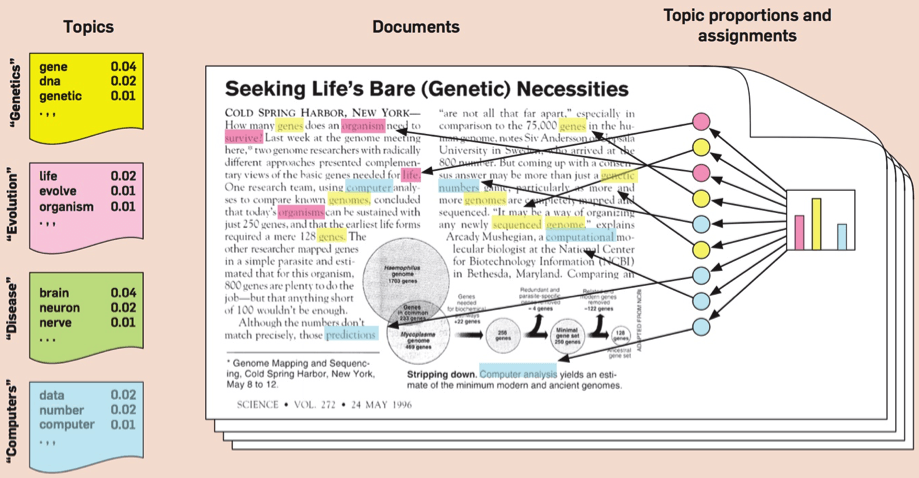
\includegraphics[scale=0.5]{chap2-img/topic_model_example2}
	\caption{نمونه‌ای از یک مدل‌سازی موضوعی}
	\label{fig2}
\end{figure}


\section{آنالیز احساس}
منظور از آنالیز احساس یا کاوش عقاید مشخص کردن اطلاعات مفهومی‌\LTRfootnote{Subjective Information}
مانند نظرات، نگرش‌ها و احساس موجود در متن نوشته شده است. در آنالیز احساس در حوزه‌ی ‌‌پردازش زبان طبیعی و پردازش متن ما به دنبال ابزار هایی هستیم که این اطلاعات مفهومی‌ را به صورت خود کار از متن یا مجموعه اسناد استخراج کند و احساس موجود در متن را برای ما مشخص کند
\cite{lin2012weakly}\cite{pang2008opinion}.
 می‌توان احساس موجود در یک متن را در سه‌ دسته قرار داد: مثبت، منفی‌ و بی‌طرف.

هدف نهایی در آنالیز احساس مشخص کردن همین امر است  که یک متن از نظر احساسی‌ مثبت، منفی‌ و یا بی‌ طرف است. در بحث تشخیص همزمان موضوعی و احساس از یک متن فرض بر این است که در یک سند متنی در مورد چندین موضوع صحبت شده است و هرکدام از این موضوع‌ها می‌‌توانند احساس خاص مربوط به خود را داشته باشند. به طور مثال فرض کنید که شما یک محصول الکترونیکی جدید مانند لپ‌تاپ خریداری کرده‌اید. حال اگر شما یک بازبینی\LTRfootnote{Review}
برای این لپ‌تاپ بنویسید، این نوشته شامل موضوعات مختلفی‌ خواهد بود چرا که یک لپ‌تاپ شامل بخش‌های مختلفی‌ نظیر صفحه نمایش، باطری، حافظه و ... است و در بازبینی نوشته شده هر کدام از این‌ها به عنوان یک موضوع مجزا در نظر گرفته می‌‌شوند. حال هرکدام از این موضوع‌ها می‌‌توانند احساس خاص مربوط به خود را داشته باشند، به طور مثال شما از حافظه لپ‌تاپ راضی‌ هستید ولی‌ در مقابل صفحه نمایش آن انتظارات شما را برآورده نکرده است، در اینجا احساس شما به موضوع حافظه مثبت و به موضوع صفحه نمایش منفی‌ خواهد بود. هدف ما در تشخیص همزمان موضوع و احساس از داده‌های متنی نیز به همین شکل می‌باشد که علاوه بر تشخیص موضوع‌های مورد بحث، احساس همراه با هرکدام را نیز تشخیص دهیم.


